\documentclass[11pt,a4paper]{article}
\usepackage[T1]{fontenc}
\usepackage{lmodern}
\usepackage[margin=2.5cm]{geometry}
\usepackage{microtype}
\usepackage{graphicx}
\usepackage{booktabs}
\usepackage{subcaption}
\usepackage{placeins}
\usepackage[font=small,labelfont=bf]{caption}
\usepackage[numbers,sort&compress]{natbib}
\usepackage{xurl}
\usepackage[hidelinks]{hyperref}
\graphicspath{{figures/}{../results/}}
% Generated by `uv run python -m atlas.paper_numbers`: do not edit by hand.
\newcommand{\zonesTotal}{6{,}976}
\newcommand{\zonesQone}{1{,}395}
\newcommand{\glasgowQone}{339}
\newcommand{\glasgowQonePct}{45}
\newcommand{\glasgowShareOfQone}{24}
\newcommand{\aeAttendances}{1{,}652{,}428}
\newcommand{\aeYear}{2025}
\newcommand{\itemsMillions}{113.2}
\newcommand{\aeFirstYear}{2018}
\newcommand{\aeLastYear}{2025}
\newcommand{\aeQone}{380}
\newcommand{\aeQfive}{200}
\newcommand{\aeRatio}{1.90}
\newcommand{\aeRatioMin}{1.90}
\newcommand{\aeRatioMax}{2.09}
\newcommand{\aeRatioFirst}{2.02}
\newcommand{\aeRatioExcess}{2.10}
\newcommand{\aeRatioFloor}{1.53}
\newcommand{\aeRatioCeiling}{2.14}
\newcommand{\unknownFirst}{0.55}
\newcommand{\unknownLast}{3.3}
\newcommand{\unknownFold}{6}
\newcommand{\aeTypeoneMin}{2.10}
\newcommand{\aeTypeoneMax}{2.29}
\newcommand{\trendFirst}{2015}
\newcommand{\trendLast}{2024}
\newcommand{\poisonFirst}{663}
\newcommand{\poisonPeak}{1{,}373}
\newcommand{\poisonPeakYear}{2020}
\newcommand{\poisonLast}{1{,}045}
\newcommand{\poisonRateFirst}{12.7}
\newcommand{\poisonRatePeak}{25.9}
\newcommand{\poisonRateLast}{19.1}
\newcommand{\fallsFirst}{787}
\newcommand{\fallsLast}{1{,}290}
\newcommand{\fallsRateFirst}{15.7}
\newcommand{\fallsRateLast}{21.9}
\newcommand{\fallsRateRise}{40}
\newcommand{\agePeriod}{2020 to 2024}
\newcommand{\fallsDeathsYear}{1{,}111}
\newcommand{\poisonDeathsYear}{1{,}197}
\newcommand{\fallsOldShare}{87}
\newcommand{\poisonMidShare}{90}
\newcommand{\fallsWomenShare}{57}
\newcommand{\poisonMenShare}{70}
\newcommand{\admFirstYear}{2015/16}
\newcommand{\admLastYear}{2024/25}
\newcommand{\admRateFirst}{1{,}067}
\newcommand{\admRateLast}{961}
\newcommand{\admEventsLast}{54{,}922}
\newcommand{\fallsAdmShare}{67}
\newcommand{\fallsOldRateFirst}{3{,}566}
\newcommand{\fallsMidRate}{964}
\newcommand{\fallsOldRate}{3{,}573}
\newcommand{\fallsYoungRate}{270}
\newcommand{\councilPeriod}{2020 to 2024}
\newcommand{\fallsPeriod}{2020/21 to 2024/25}
\newcommand{\scotPoison}{22.2}
\newcommand{\scotFalls}{652}
\newcommand{\aboveCount}{8}
\newcommand{\belowCount}{14}
\newcommand{\aboveQone}{37}
\newcommand{\belowQone}{6}
\newcommand{\fallsAboveCount}{12}
\newcommand{\fallsBelowCount}{14}
\newcommand{\fallsAboveQone}{24}
\newcommand{\fallsBelowQone}{9}
\newcommand{\rhoPoison}{0.91}
\newcommand{\rhoAllDeaths}{0.85}
\newcommand{\rhoFalls}{0.53}
\newcommand{\rhoAllAdm}{0.46}
\newcommand{\fewCount}{3}
\newcommand{\fewNames}{Na h-Eileanan Siar, Orkney Islands, Shetland Islands}
\newcommand{\itemsQone}{30.2}
\newcommand{\itemsQfive}{10.7}
\newcommand{\pharmQone}{3.2}
\newcommand{\pharmQfive}{1.4}
\newcommand{\rhoItems}{0.40}
\newcommand{\cnsQone}{21.2}
\newcommand{\cnsQfive}{16.8}
\newcommand{\respQone}{7.8}
\newcommand{\respQfive}{6.6}
\newcommand{\cardioQone}{22.7}
\newcommand{\cardioQfive}{24.3}
\newcommand{\unplacedShare}{1.4}
\newcommand{\valDeaths}{2{,}822}
\newcommand{\valAdmPub}{56{,}294}
\newcommand{\valAdmOurs}{57{,}082}
\newcommand{\valAdmDiff}{1.4}
\newcommand{\valAdmLateDiff}{0.3}
\newcommand{\valWorst}{1.8}
\newcommand{\oldFallsShare}{86}
\newcommand{\valCount}{9}
\newcommand{\waitsFirstYear}{2008}
\newcommand{\waitsLastYear}{2025}
\newcommand{\waitsFirst}{97.6}
\newcommand{\waitsNineteen}{87.4}
\newcommand{\waitsLast}{65.0}
\newcommand{\waitsLastMet}{2011}
\newcommand{\overEightLast}{12.3}
\newcommand{\overTwelveFirst}{0.03}
\newcommand{\overTwelveLast}{5.3}
\newcommand{\overTwelveVisits}{75{,}000}
\newcommand{\gpHeadQone}{7.7}
\newcommand{\gpHeadQfive}{7.9}
\newcommand{\gpWteQone}{5.5}
\newcommand{\gpWteQfive}{6.4}
\newcommand{\gpWteGap}{13}
\newcommand{\gpPatients}{6{,}035{,}952}
\newcommand{\gpBoardsClose}{12}
\newcommand{\gpBoardWorst}{0.25}
\newcommand{\gpQonePerGp}{1{,}293}
\newcommand{\gpQfivePerGp}{1{,}264}
\newcommand{\gpQonePerWte}{1{,}810}
\newcommand{\gpQfivePerWte}{1{,}575}
\newcommand{\gpScenGap}{2.3}
\newcommand{\gpScenExtra}{102}
\newcommand{\gpScenSessions}{814}
\newcommand{\fallsDeathsUnplaced}{82}
\newcommand{\poisonDeathsHome}{87}
\newcommand{\fallsAdmHomePlaced}{70}
\newcommand{\costQone}{11.00}
\newcommand{\costQfive}{12.21}
\newcommand{\costMidLow}{10.57}

% table rows from generated files (LaTeX's \input cannot come just before \bottomrule)
\makeatletter\newcommand{\rows}[1]{\@@input #1 }\makeatother

\title{Where you live and how old you are: a reproducible atlas of A\&E use, unintentional
injuries and prescribing in Scotland}
\author{David Obeh Alobo\\[2pt]
  \small Monstrous Data, \href{mailto:david.alobo@monstrous.com.ng}{david.alobo@monstrous.com.ng}}
\date{}

\begin{document}
\maketitle

\begin{abstract}
\noindent
We describe how A\&E attendances, emergency admissions and deaths from unintentional injuries, and
community prescribing in Scotland vary with neighbourhood deprivation and age, using the open data
package released by Public Health Scotland for The Data Lab's 2026 visualisation competition,
together with national population estimates and the Scottish Index of Multiple Deprivation. Rates
were standardised for age and sex, and every number in this paper is generated from saved results
tables. In \aeLastYear{}, people living in the most deprived fifth of neighbourhoods attended A\&E
\aeQone{} times per 1{,}000 against \aeQfive{} in the least deprived fifth, a ratio of \aeRatio{};
the ratio stayed between \aeRatioMin{} and \aeRatioMax{} from \aeFirstYear{} to \aeLastYear{}. A
slight fall in the ratio over these years lies within what the growing share of attendances with
unknown deprivation can produce, so we do not claim that the gap narrowed. Deaths from accidental
poisoning rose from \poisonRateFirst{} to \poisonRatePeak{} per 100{,}000 between \trendFirst{} and
\poisonPeakYear{} and fell back to \poisonRateLast{} in \trendLast{}. Across the 32 council areas,
their rate followed the share of people in the most deprived fifth closely (Spearman's
$\rho = \rhoPoison$), while falls admissions followed it less ($\rho = \rhoFalls$). Falls instead
follow age: \fallsOldShare\% of deaths after a fall were of people aged 75 or over, while
\poisonMidShare\% of poisoning deaths were at ages 25 to 64. Our counts reproduce Public Health
Scotland's published figures within \valWorst\%. The analysis is descriptive, and the comparisons
between council areas describe areas rather than people. The results are also published as a
scrolling web atlas in which a reader can find their own neighbourhood.
\end{abstract}

\section{Introduction}

Scotland has had higher mortality than the rest of Western Europe for decades, and Glasgow higher
mortality than similarly deprived cities elsewhere in Britain \citep{walsh2017}. Deaths of people who
use drugs make up a substantial part of Scotland's excess mortality \citep{bloor2008},
and National Records of Scotland reported that in 2023 people in the most deprived areas were 15.3
times more likely to die of drug misuse than people in the least deprived areas
\citep{nrsdrugs2024}. At the other end of life, falls account for about \oldFallsShare\% of emergency
admissions for unintentional injuries at ages 65 and over \citep{phsinjuries2024}, and their
prevention is organised around age and frailty rather than place \citep{montero2022}.
In England, practices serving more deprived populations have higher A\&E attendance rates
\citep{scantlebury2015}.

In September 2026 Public Health Scotland released a data package for The Data Lab's data
visualisation competition, with the theme ``Telling Scotland's health story'' \citep{datalab2026}.
The package holds A\&E attendances by site and by deprivation, emergency admissions and deaths from
unintentional injuries by council area, and community prescribing by dispensing location. These
datasets are already published separately on the Scottish Health and Social Care Open Data
platform \citep{phsopendata}, but they are rarely brought together on the same denominators.

Our aim was to use this package to ask two simple questions. First, how much does where you live,
measured as neighbourhood deprivation, change how often people use A\&E, are admitted or die after an
unintentional injury, and receive medicines? Second, for which of these outcomes does age matter more
than place? To answer them we built every rate from national population estimates, standardised for
age and sex, checked our counts against Public Health Scotland's own publications, and kept every
step as code with saved results. We then turned the results into a scrolling web atlas, following
the ideas of narrative visualisation \citep{segel2010}, so that a reader can see the same numbers
for their own neighbourhood. This paper describes the data, methods and results behind that atlas.

\section{Data and methods}

Figure~\ref{fig:design} shows the study design. All analyses were done in Python with DuckDB; the
code, the saved results tables and the atlas are openly available (Section~\ref{sec:availability}).

\begin{figure}[t]
  \centering
  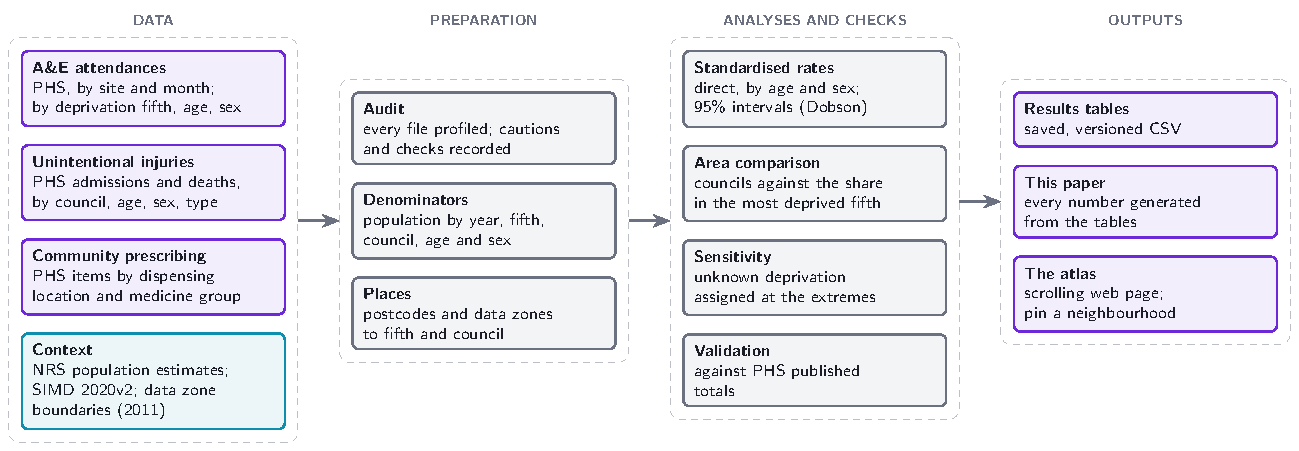
\includegraphics[width=\textwidth]{design.pdf}
  \caption{Study design. Three Public Health Scotland datasets and the national context data were
    profiled, given population denominators and placed in deprivation fifths and council areas.
    Standardised rates, comparisons between council areas, a sensitivity analysis and a validation
    against published figures were saved as tables, from which this paper and the atlas are
    generated.}
  \label{fig:design}
\end{figure}

\subsection{Data}

The competition package \citep{datalab2026} contains four sets of files. The A\&E activity file gives
monthly attendances at 103 sites from July 2007 to June 2026. The A\&E demographics file gives
monthly attendances for the 14 health boards from January 2018 to June 2026, by age band, sex and
the deprivation quintile of the patient's postcode. The unintentional injury files give emergency
admissions for financial years 2015/16 to 2024/25 and deaths for calendar years 2015 to 2024, by
council area, age band, sex, injury type and place of injury. The prescribing files give items
dispensed in the community by month, dispensing location and chapter of the British National
Formulary, from 2019 to May 2026. Before any analysis we profiled every file and recorded its
columns, ranges, missing values and suppressed cells.

To these we added the Scottish Index of Multiple Deprivation 2020 (version 2) look-ups for data
zones and postcodes \citep{simd2020}, the 2011 data zone boundaries, and the National Records of
Scotland small area population estimates on 2011 data zones \citep{nrssape}. Scotland has
\zonesTotal{} data zones, each with about 800 residents; \zonesQone{} of them form the most deprived
fifth (quintile~1). Because the deprivation index is defined on 2011 data zones, we used the
population estimates on the same zones: the rebased estimates for mid-2011 to mid-2021 and the
estimates for mid-2023 and mid-2024. Mid-2022 is not published on 2011 data zones, so we took the
mean of mid-2021 and mid-2023; years after 2024 use mid-2024.

\subsection{Rates and standardisation}

For A\&E, attendances in each whole calendar year from \aeFirstYear{} to \aeLastYear{} were summed
over all boards by deprivation quintile, age band and sex, and divided by the population of the same
quintile, age band and sex. Rates per 1{,}000 people were directly standardised for age and sex to
Scotland's mid-2024 population. We used national rates, so a patient attending a hospital in
another board is still counted with their own neighbourhood. Attendances with unknown deprivation,
age or sex were left out of the quintile rates, and their share was recorded. The main analysis used
all sites (emergency departments and minor injury units); we repeated it for emergency departments
alone.

For injuries, rates per 100{,}000 people were standardised for age and sex to the 2013 European
Standard Population \citep{esp2013}, as Public Health Scotland does, with its five-year bands summed
to the eight age bands of the files. Confidence intervals (95\%) were calculated by the method of
Dobson and colleagues \citep{dobson1991}, with Byar's approximation for the count. A financial year
took the population of the year it starts in. Council rates pool the latest five years (admissions
\fallsPeriod{}, deaths \councilPeriod{}), since most single years of a council have few events. A
council was called above or below Scotland when its interval excluded the Scotland rate. These are
32 comparisons for each outcome, not corrected for multiplicity, and we read them as descriptive. In
the atlas, rates based on fewer than 20 deaths are shown hatched and not given a colour.

\subsection{Deprivation in the injury and prescribing data}

The injury files do not record deprivation. We therefore compared council areas: each council's
standardised rate against the share of its population living in quintile~1 data zones (mid-2024),
summarised by Spearman's rank correlation with average ranks for ties. This is an ecological
comparison. It describes areas, and a correlation between areas does not show that the same
relation holds for the people in them \citep{robinson1950}.

For prescribing, each dispensing location's postcode was placed in its data zone, and so in a
deprivation quintile and council area. This counts where medicines are dispensed, not where patients
live. Items were divided by the mid-2024 population of the same quintile; the files carry no age, so
these rates are not standardised. Some location codes have no address, and their share of items fell
from about a quarter in 2019 to \unplacedShare\% in the latest twelve months (June 2025 to May
2026), so we used only those twelve months. We also compared the medicine mix as each chapter's
share of a quintile's items, which does not depend on population or on where pharmacies are.

\subsection{Sensitivity analysis and validation}

The share of A\&E attendances with unknown deprivation, but known age and sex, rose from
\unknownFirst\% in \aeFirstYear{} to \unknownLast\% in \aeLastYear{}. To see how far this could move
the ratio between the most and least deprived fifths, we assigned all of these attendances, within
each age and sex group, first to quintile~1 and then to quintile~5, and re-standardised. In a third
scenario only the growth in unknown attendances since 2018--2019 was assigned to quintile~1.

To check the injury pipeline we compared \valCount{} of our counts, shares and rates with those
published by Public Health Scotland for 2023/24 and 2024/25 \citep{phsinjuries2024}.

\subsection{The atlas}

The atlas is a single web page written in plain JavaScript, with no build step. Each of the
\zonesTotal{} data zones is drawn as a dot at its centre, with brightness by deprivation, and the
story moves through fifteen scenes as the reader scrolls. A reader can search by postcode or
neighbourhood name, or click a dot, to pin a neighbourhood; the panels then show that
neighbourhood's deprivation, its council's rates beside Scotland's, and the deaths in its council by
age. The data behind the page are exported from the same results tables as this paper.

\section{Results}

\subsection{Where the most deprived neighbourhoods are}

The most deprived fifth of data zones is concentrated in the west of the Central Belt
(Figure~\ref{fig:atlas}a). Glasgow City alone holds \glasgowQone{} of the \zonesQone{} most deprived
zones, which is \glasgowShareOfQone\% of them and \glasgowQonePct\% of the city's own zones.

\begin{figure}[t]
  \centering
  \begin{subfigure}{0.49\textwidth}
    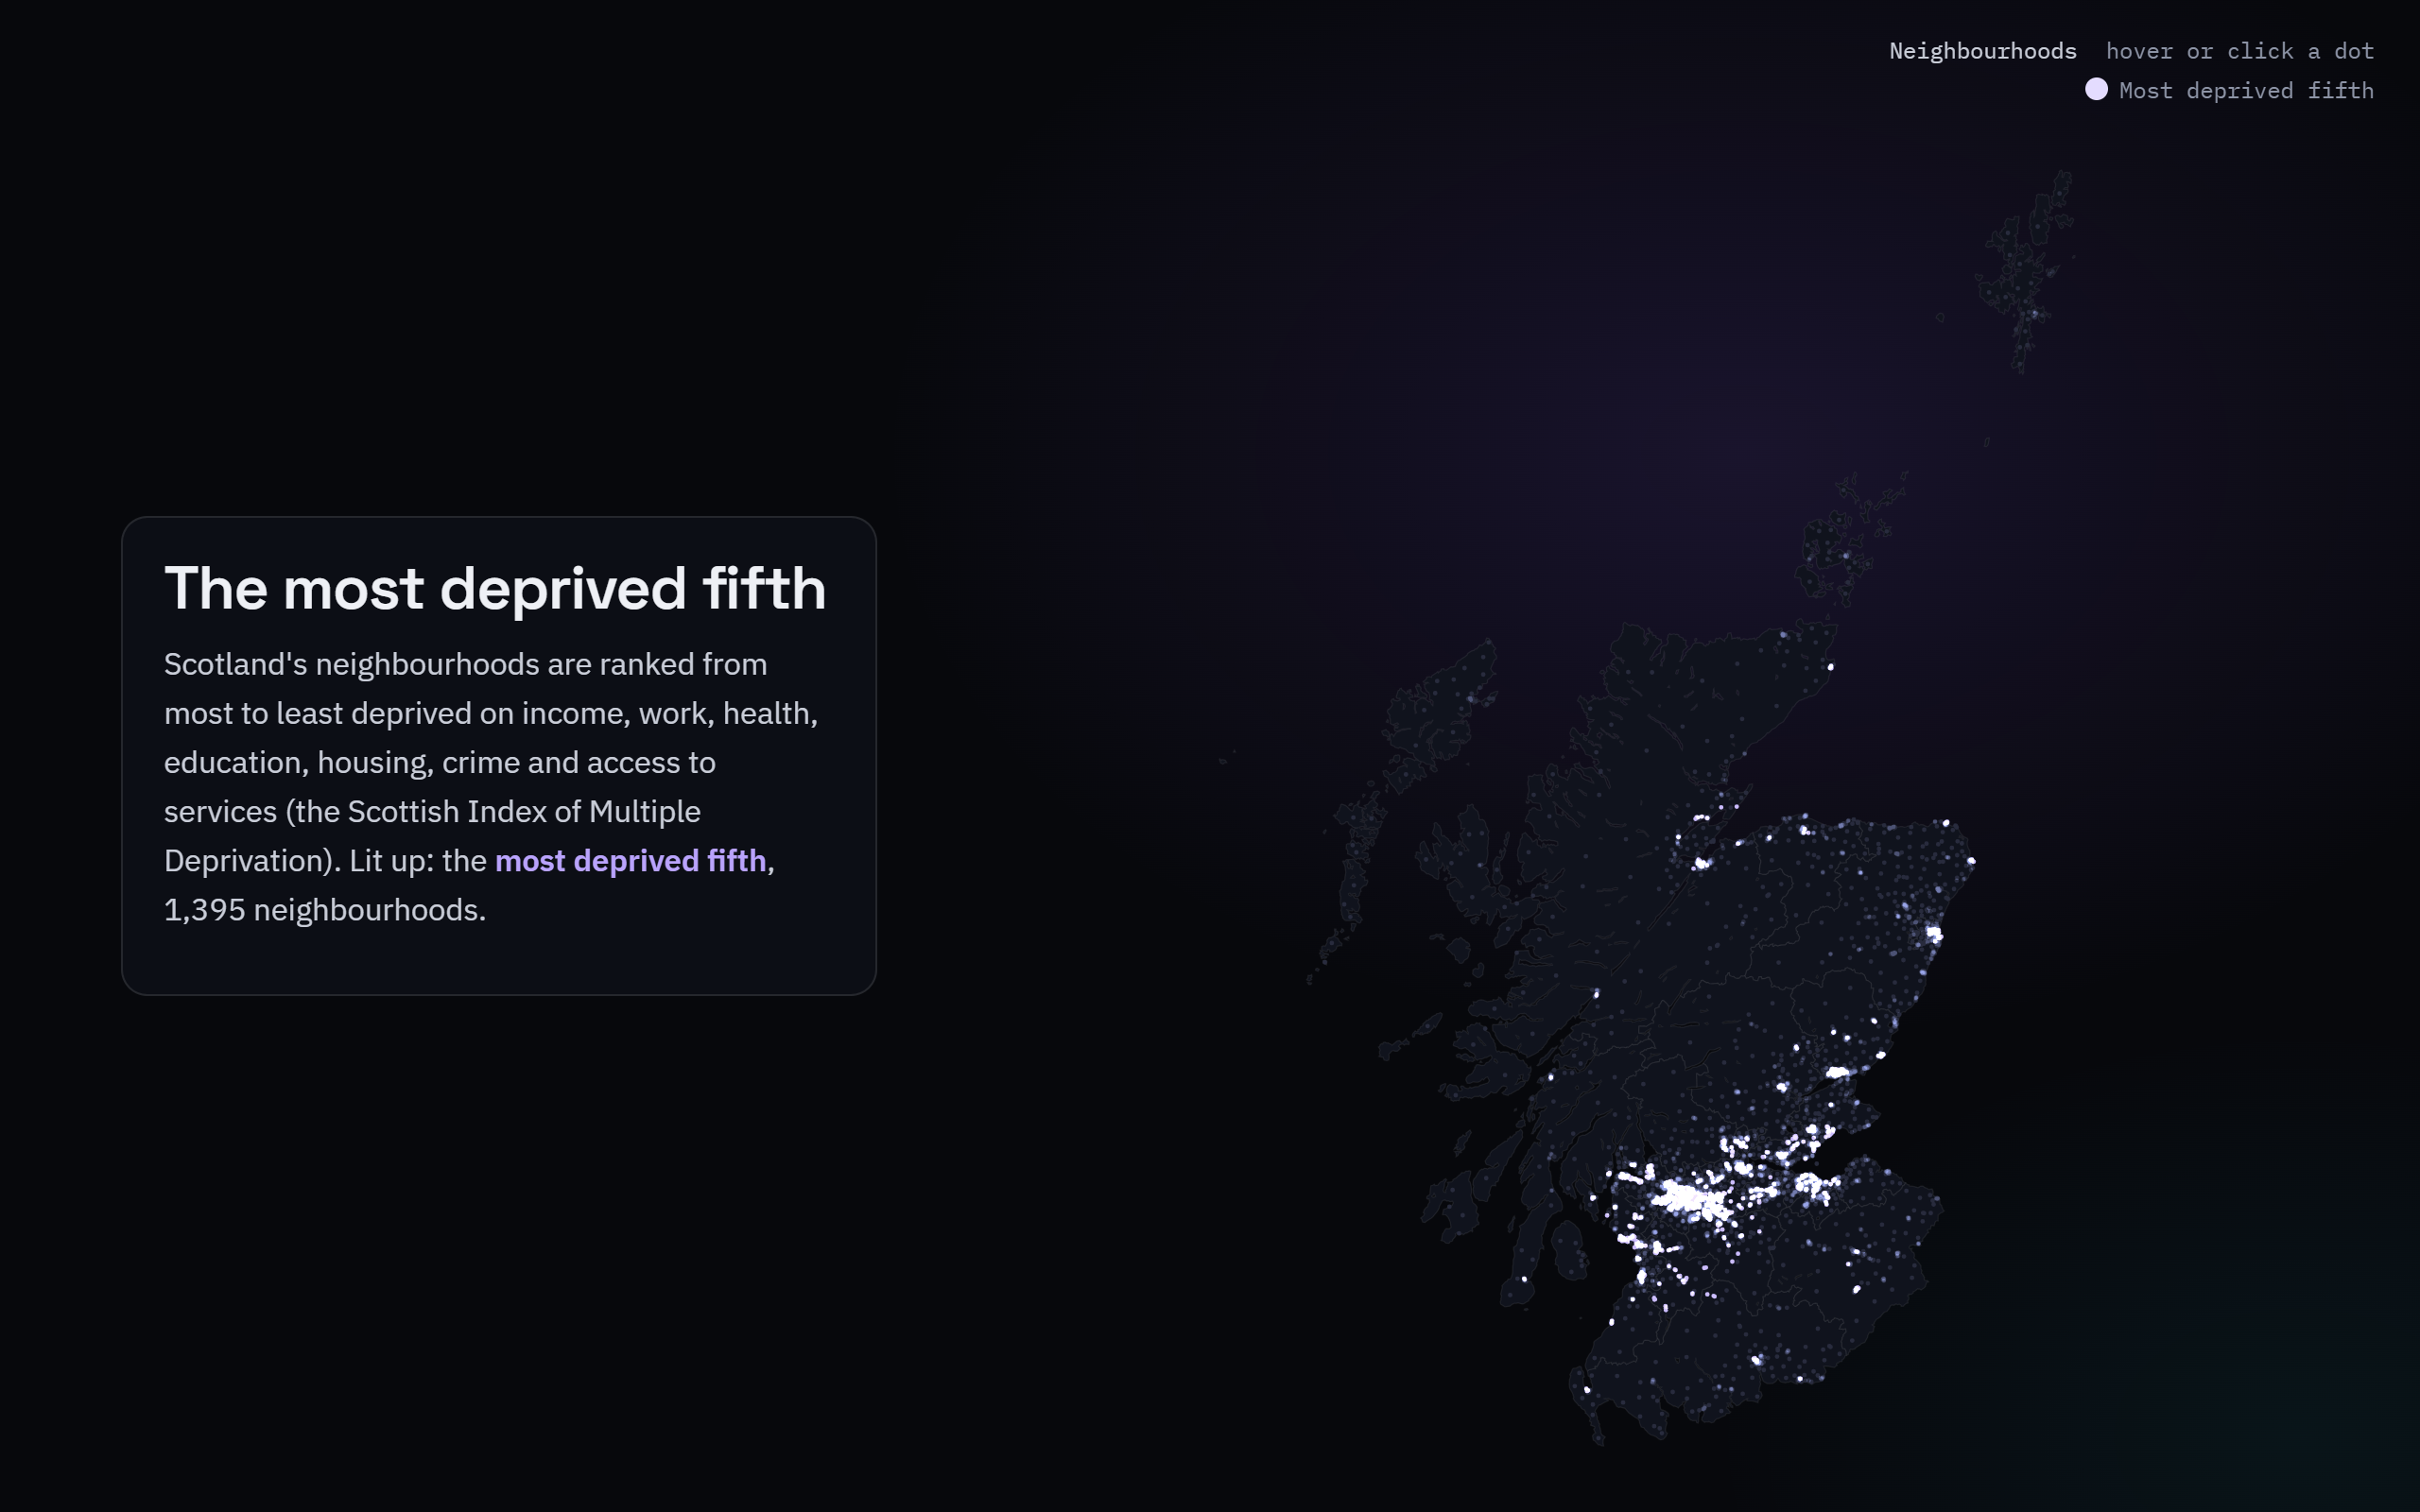
\includegraphics[width=\textwidth]{atlas-deprived.png}
    \caption{}
  \end{subfigure}\hfill
  \begin{subfigure}{0.49\textwidth}
    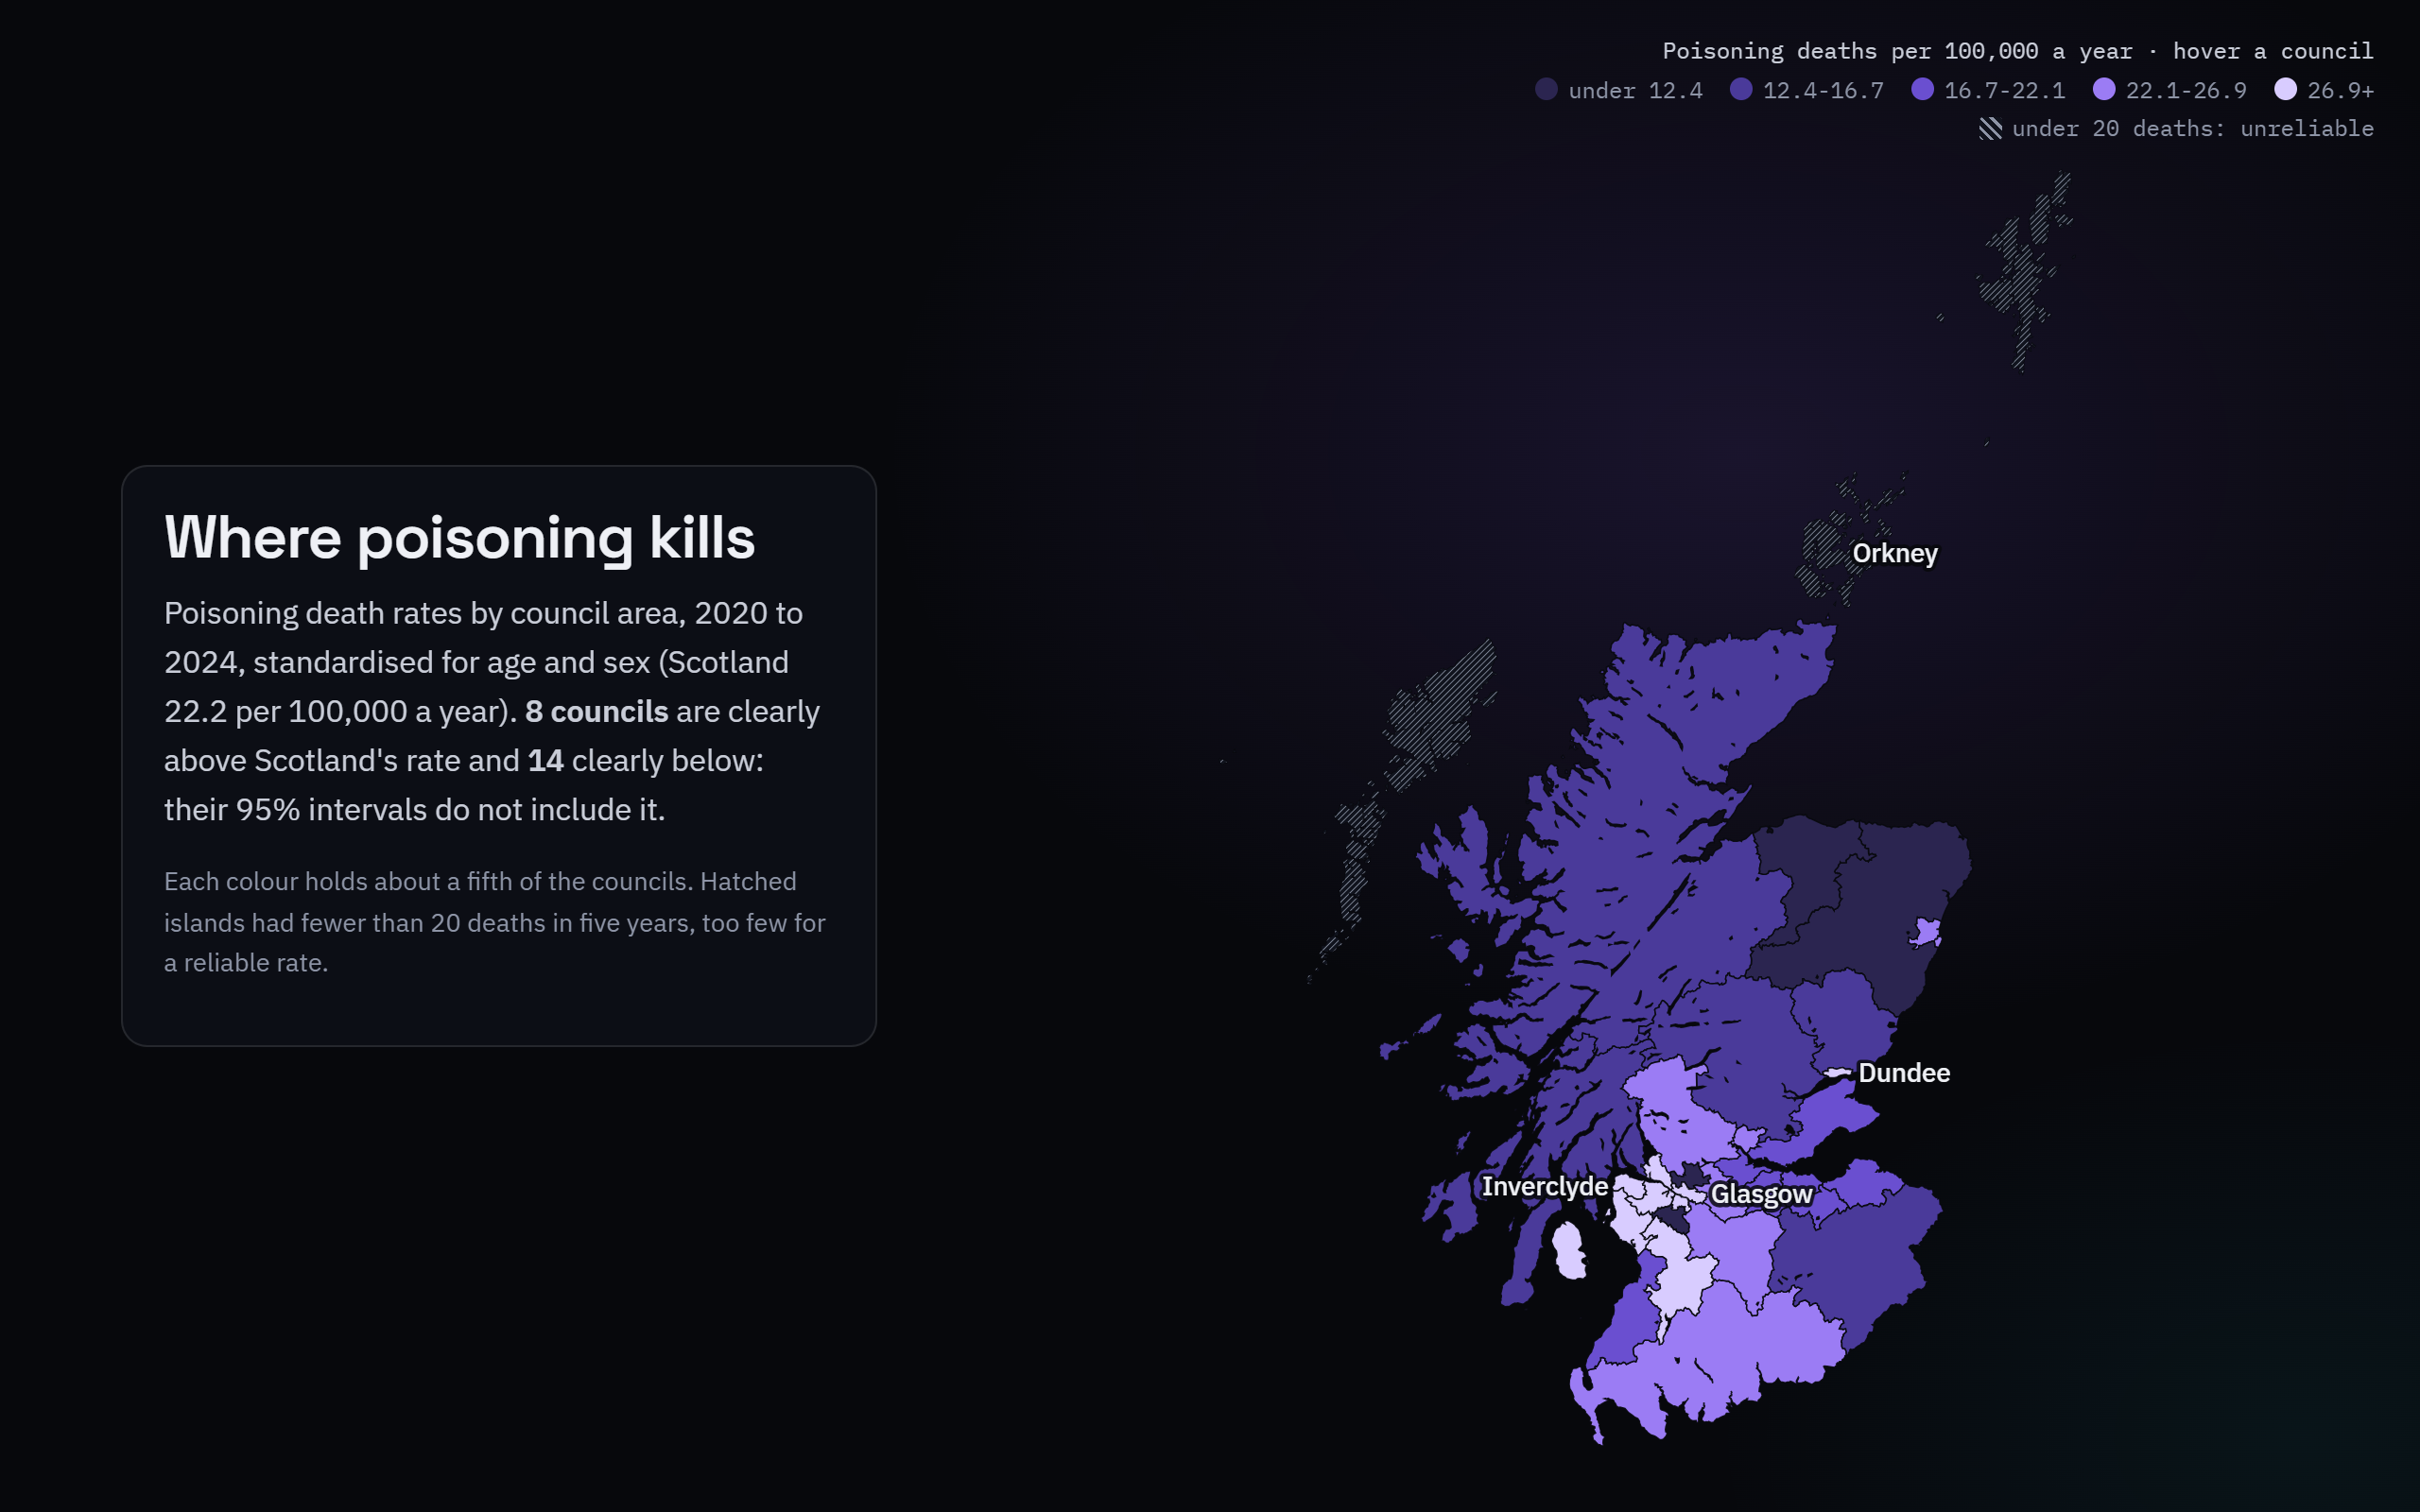
\includegraphics[width=\textwidth]{atlas-poison.png}
    \caption{}
  \end{subfigure}
  \caption{Two scenes of the web atlas: (a) the \zonesQone{} most deprived data zones lit among
    Scotland's \zonesTotal; (b) poisoning death rates by council area, \councilPeriod, with the
    island councils with fewer than 20 deaths hatched.}
  \label{fig:atlas}
\end{figure}

\subsection{A\&E attendances}

In every year from \aeFirstYear{} to \aeLastYear{}, people in more deprived neighbourhoods attended
A\&E more often than people of the same age and sex in less deprived ones, and each step in
deprivation brought more attendances (Figure~\ref{fig:ae}). In \aeLastYear{} the standardised rate
was \aeQone{} attendances per 1{,}000 people in the most deprived fifth and \aeQfive{} in the least
deprived fifth, a ratio of \aeRatio{}. Over the eight years the ratio ranged from \aeRatioMin{} to
\aeRatioMax{}. At emergency departments alone the ratio was higher, between \aeTypeoneMin{} and
\aeTypeoneMax{}. All quintiles fell in 2020 and recovered afterwards. In \aeLastYear{} Scotland's
sites recorded \aeAttendances{} attendances.

\begin{figure}[t]
  \centering
  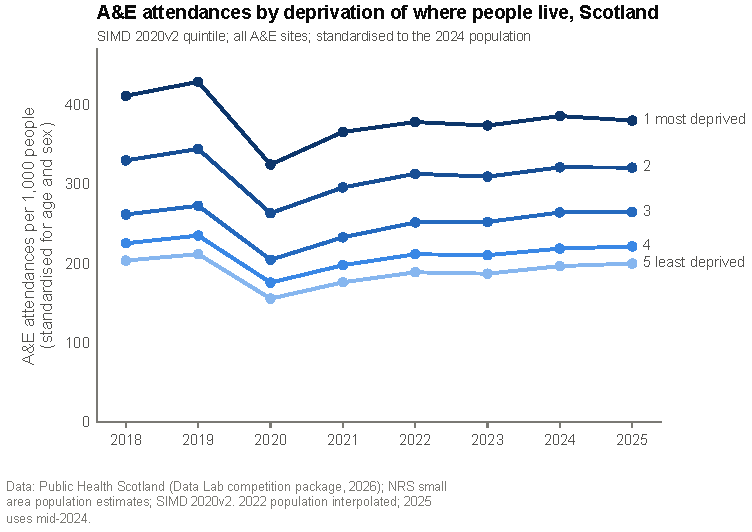
\includegraphics[width=0.72\textwidth]{2026-11-14-ae-deprivation/rates.pdf}
  \caption{A\&E attendances per 1{,}000 people by deprivation quintile of the patient's
    neighbourhood, \aeFirstYear{} to \aeLastYear{}, all sites, standardised for age and sex to
    Scotland's mid-2024 population.}
  \label{fig:ae}
\end{figure}

The ratio fell from \aeRatioFirst{} in \aeFirstYear{} to \aeRatio{} in \aeLastYear{}. Over the same
years the share of attendances with unknown deprivation grew about \unknownFold-fold. When all of the
\aeLastYear{} unknowns were assigned to the most deprived fifth the ratio was \aeRatioCeiling{}, and
when they were all assigned to the least deprived fifth it was \aeRatioFloor{}. If only the growth in
unknowns since 2018--2019 came from the most deprived fifth, the ratio would be \aeRatioExcess{},
level with the earlier years. The fall in the ratio is therefore within what the missing data can
produce, and we do not claim that the gap narrowed. Even in the least favourable scenario the most
deprived fifth attended \aeRatioFloor{} times as often as the least deprived.

\subsection{Unintentional injuries over time}

Emergency admissions for unintentional injuries fell from \admRateFirst{} per 100{,}000 in
\admFirstYear{} to \admRateLast{} in \admLastYear{} (\admEventsLast{} admissions in the latest year),
and falls made up \fallsAdmShare\% of them (Figure~\ref{fig:trend}a). Deaths followed two different
paths (Figure~\ref{fig:trend}b). Deaths from poisoning rose from \poisonFirst{} (\poisonRateFirst{}
per 100{,}000) in \trendFirst{} to \poisonPeak{} (\poisonRatePeak) in \poisonPeakYear, then fell to
\poisonLast{} (\poisonRateLast) in \trendLast. Deaths after a fall rose steadily, from \fallsFirst{}
(\fallsRateFirst) to \fallsLast{} (\fallsRateLast). Because these rates are standardised, the rise
in falls deaths is not only the result of an older population.

\begin{figure}[t]
  \centering
  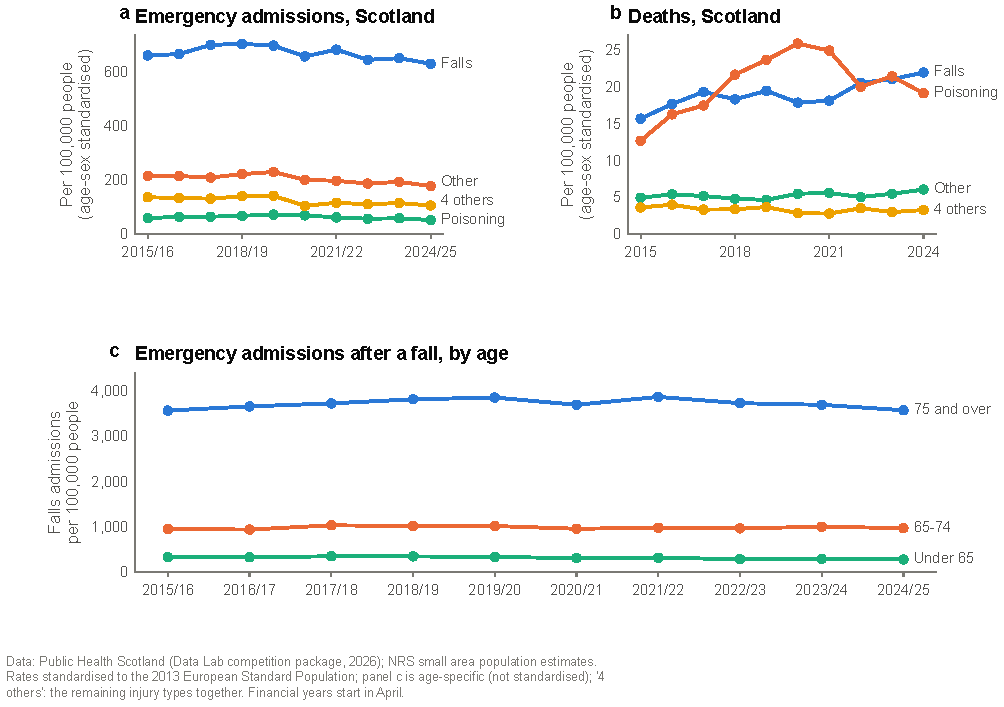
\includegraphics[width=0.95\textwidth]{2026-11-14-injuries/national.pdf}
  \caption{Unintentional injuries in Scotland: (a) emergency admissions and (b) deaths by injury
    type, standardised for age and sex to the 2013 European Standard Population; (c) falls
    admissions by age band (age-specific rates).}
  \label{fig:trend}
\end{figure}

\subsection{Falls and poisoning by age}

Falls and poisoning affect people at different stages of life (Figure~\ref{fig:age}). From
\agePeriod{}, an average of \fallsDeathsYear{} people a year died after a fall; \fallsOldShare\% of
them were aged 75 or over and \fallsWomenShare\% were women. An average of \poisonDeathsYear{} a year
died of poisoning; \poisonMidShare\% were aged 25 to 64 and \poisonMenShare\% were men. In
\admLastYear{} the falls admission rate was \fallsOldRate{} per 100{,}000 at ages 75 and over,
\fallsMidRate{} at 65 to 74 and \fallsYoungRate{} under 65. The rate at 75 and over was much the same
in \admFirstYear{} (\fallsOldRateFirst), so the number of falls admissions has followed the size of
the oldest age group.

\begin{figure}[t]
  \centering
  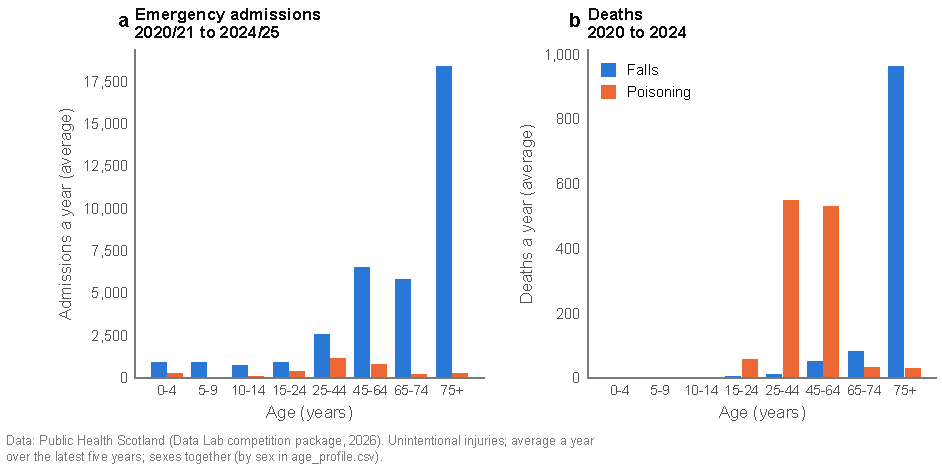
\includegraphics[width=0.9\textwidth]{2026-11-14-injuries/age_profile.pdf}
  \caption{Emergency admissions and deaths a year by age band, falls against poisoning, Scotland,
    latest five years.}
  \label{fig:age}
\end{figure}

\subsection{Council areas}

Deaths from poisoning in \councilPeriod{} averaged \scotPoison{} per 100{,}000 a year in Scotland,
standardised. Of the 32 councils, \aboveCount{} had a rate whose interval lay above Scotland's and
\belowCount{} below (Figure~\ref{fig:councils}a; Table~\ref{tab:councils}). On average
\aboveQone\% of the people in the councils above Scotland lived in the most deprived fifth, against
\belowQone\% in the councils below. Across all councils, the rank correlation between the poisoning
death rate and the share in the most deprived fifth was \rhoPoison{} (\rhoAllDeaths{} for all
unintentional injury deaths; Figure~\ref{fig:eco}). Three island councils (\fewNames) had fewer than
20 poisoning deaths in the five years, and their rates are uncertain.

\begin{table}[t]
  \centering
  \caption{Council areas whose poisoning death rate was above Scotland's (\scotPoison{} per
    100{,}000 a year), \councilPeriod{}, standardised for age and sex. Q1 share: people living in
    the most deprived fifth of data zones. Falls admissions per 100{,}000 a year, \fallsPeriod{}
    (Scotland \scotFalls).}
  \label{tab:councils}
  \small
  \begin{tabular}{lrcrr}
    \toprule
    Council & Poisoning deaths & 95\% interval & Q1 share (\%) & Falls admissions \\
    \midrule
    \rows{generated/table_councils.tex}
    \bottomrule
  \end{tabular}
\end{table}

Falls admissions in \fallsPeriod{} averaged \scotFalls{} per 100{,}000 a year. \fallsAboveCount{}
councils were above Scotland and \fallsBelowCount{} below, and the councils above had on average
\fallsAboveQone\% of their people in the most deprived fifth, against \fallsBelowQone\% for those
below. The rank correlation with the deprived share was weaker than for poisoning, \rhoFalls{}
(\rhoAllAdm{} for all admissions). Several rural councils with few people in the most deprived
fifth had falls admission rates above Scotland's, which suggests that falls admissions depend on
something besides deprivation, for example the age of the population or local admission practice.
Our data cannot separate these.

\begin{figure}[t]
  \centering
  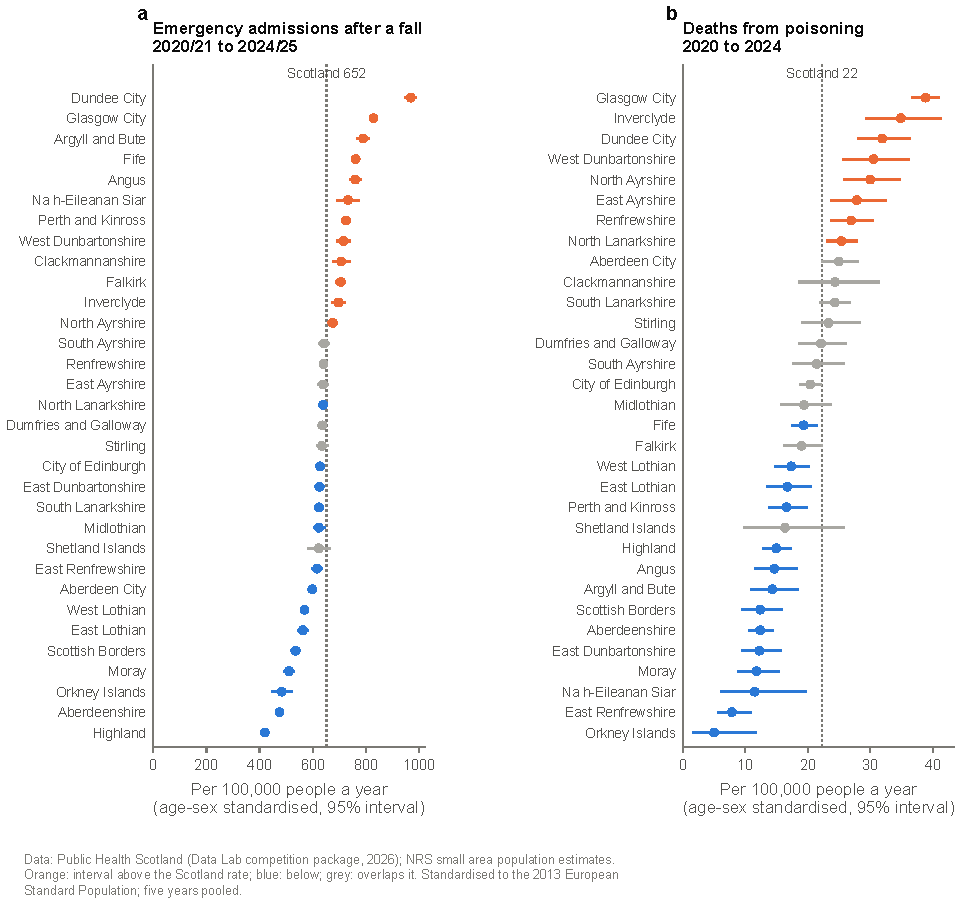
\includegraphics[width=0.9\textwidth]{2026-11-14-injuries/councils.pdf}
  \caption{Council rates with 95\% intervals: (a) falls admissions, \fallsPeriod{}, and (b)
    poisoning deaths, \councilPeriod{}, per 100{,}000 a year, standardised for age and sex. The
    vertical line is Scotland's rate.}
  \label{fig:councils}
\end{figure}

\begin{figure}[t]
  \centering
  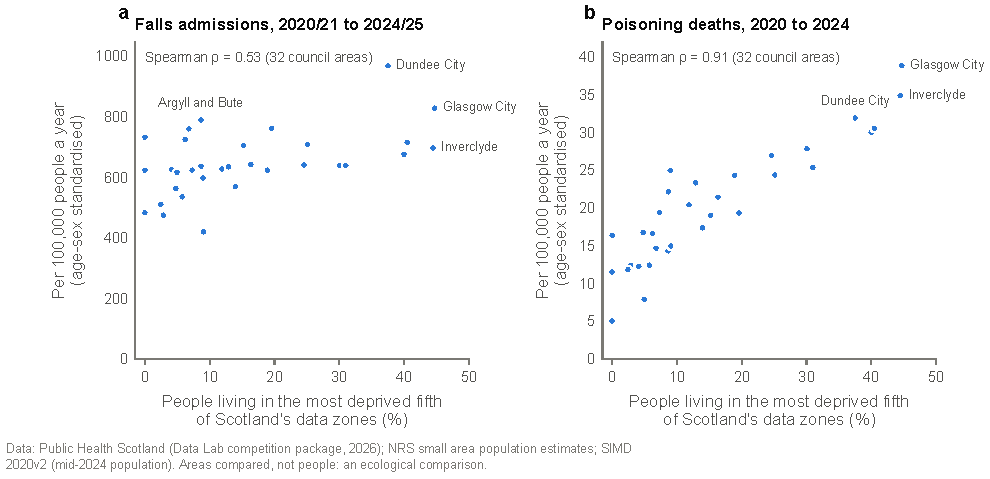
\includegraphics[width=0.95\textwidth]{2026-11-14-injuries/ecological.pdf}
  \caption{Council rates against the share of each council's people living in the most deprived
    fifth of data zones (32 councils). The comparison is between areas, not people.}
  \label{fig:eco}
\end{figure}

\subsection{Prescribing}

In the twelve months to May 2026, \itemsMillions{} million items were dispensed in the community.
Locations in the most deprived fifth of data zones dispensed \itemsQone{} items per person living
there, against \itemsQfive{} in the least deprived fifth (Figure~\ref{fig:rx}). However, there were
also \pharmQone{} dispensing locations per 10{,}000 people in the most deprived fifth against
\pharmQfive{} in the least, so most of this difference reflects where pharmacies are rather than
who receives the medicines. The medicine mix does not depend on where pharmacies are. Medicines for
the central nervous system made up \cnsQone\% of items in the most deprived fifth and \cnsQfive\% in
the least, and respiratory medicines \respQone\% and \respQfive\%. Cardiovascular medicines were a
smaller share in the most deprived fifth (\cardioQone\% against \cardioQfive\%), which may reflect
the older populations of less deprived areas. Across councils, items per person correlated only
weakly with the deprived share ($\rho = \rhoItems$), and these rates are not standardised for age.

\begin{figure}[t]
  \centering
  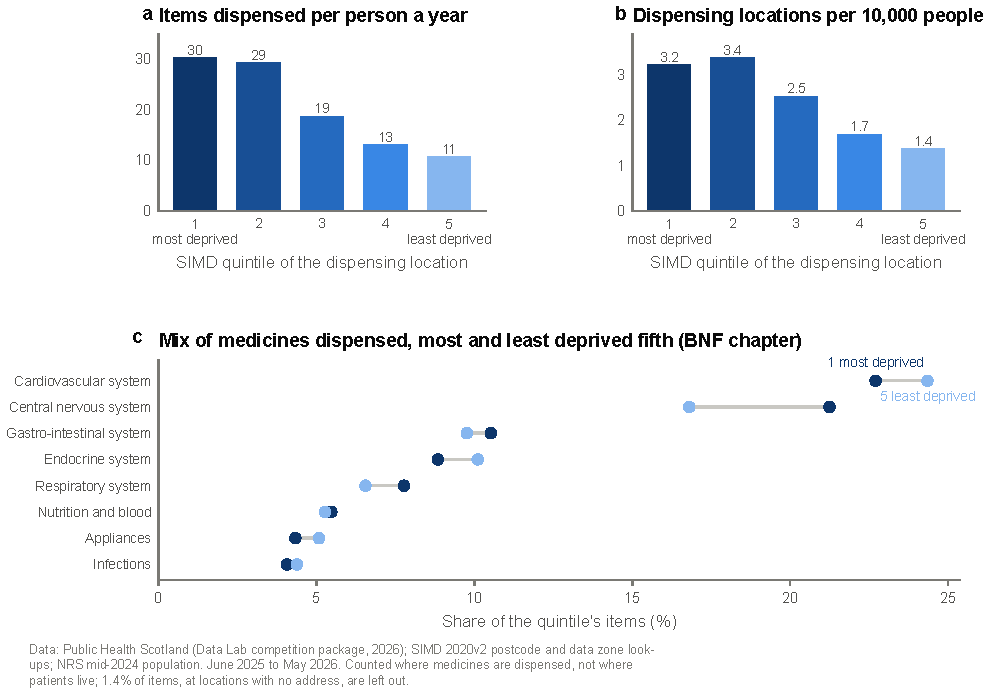
\includegraphics[width=0.95\textwidth]{2026-11-14-prescribing/quintiles.pdf}
  \caption{Community prescribing by the deprivation quintile of the dispensing location, June 2025
    to May 2026: (a) items per person, (b) dispensing locations per 10{,}000 people, (c) share of
    items by chapter of the British National Formulary, most against least deprived fifth. Not
    standardised for age.}
  \label{fig:rx}
\end{figure}

\subsection{Validation}

Our injury counts matched Public Health Scotland's published figures closely
(Table~\ref{tab:validation}). Deaths in 2023 matched exactly (\valDeaths). Admissions in 2023/24
were \valAdmOurs{} in the package against \valAdmPub{} published, \valAdmDiff\% higher, while the
2024/25 count of admissions at 65 and over agreed within \valAdmLateDiff\%. The likely reason is that records for a year keep arriving after
its first publication, so the later release revises the earlier year upwards; we have not confirmed
this with Public Health Scotland. No figure differed by more than \valWorst\%.

\begin{table}[t]
  \centering
  \caption{Injury figures from the competition package against Public Health Scotland's
    publications. EASR: rate per 100{,}000 standardised to the 2013 European Standard Population.}
  \label{tab:validation}
  \small
  \begin{tabular}{lrrr}
    \toprule
    Figure & Published & Ours & Difference (\%) \\
    \midrule
    \rows{generated/table_validation.tex}
    \bottomrule
  \end{tabular}
\end{table}

\FloatBarrier
\section{Discussion}

Figure~\ref{fig:concept} summarises what we found. Where people live was strongly related to how
often they attended A\&E and, across council areas, to deaths from poisoning. Age mattered more for
falls: deaths and admissions after a fall were concentrated in people aged 75 and over, and falls
admissions varied between councils in ways that deprivation explained only partly.

\begin{figure}[t]
  \centering
  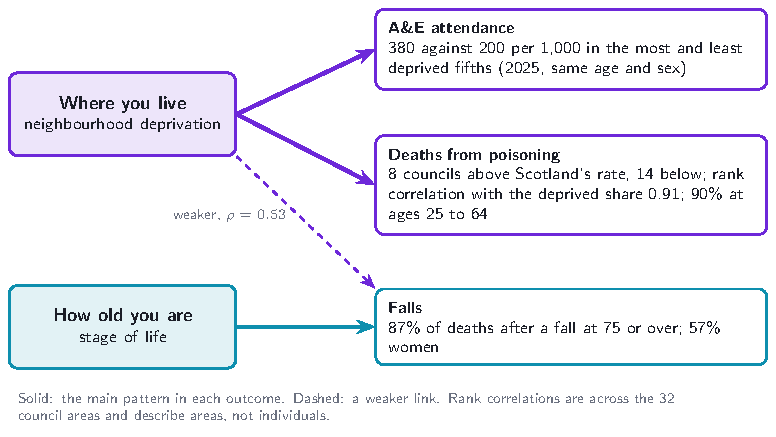
\includegraphics[width=0.85\textwidth]{concept.pdf}
  \caption{Summary of the findings. Neighbourhood deprivation was strongly related to A\&E
    attendance and, between council areas, to deaths from poisoning; age was the main pattern in
    falls.}
  \label{fig:concept}
\end{figure}

The twofold gap in A\&E attendance is in line with the English finding that practices with more
deprived populations have more attendances \citep{scantlebury2015}. Our comparison is by the
patient's neighbourhood rather than their practice, and it is standardised for age and sex, so the
gap is not explained by the most deprived areas having younger or older populations. We could not
show whether the gap is changing. The apparent narrowing since 2018 is of the same size as the
effect of the growing number of attendances with unknown deprivation, and this is a reason to report
the share of unknowns alongside any trend in the ratio.

The poisoning deaths in the injury files do not record the substance. National Records of Scotland
classified 88\% of drug misuse deaths in 2023 as accidental poisonings \citep{nrsdrugs2024}, so it is
likely that most of the poisoning deaths here are drug deaths, and their rise to \poisonPeakYear{}
and their concentration in mid-life and in the most deprived council areas match the published
picture of drug deaths in Scotland \citep{bloor2008,nrsdrugs2024}. However, we did not test this
link. Falls, in contrast, behaved as an outcome of age, which agrees with prevention guidance that
targets older adults \citep{montero2022}. The standardised falls death rate still rose by
\fallsRateRise\% from \trendFirst{} to \trendLast, so the growth is not only a matter of more older people.

This work has several limitations. First, the injury and prescribing comparisons are ecological. A
council with many deprived neighbourhoods and a high poisoning death rate does not show that the
people who died lived in those neighbourhoods \citep{robinson1950}. Second, the 32 council
comparisons for each outcome were not corrected for multiplicity and should be read as
descriptive. Third, A\&E attendances are visits, not people, and area deprivation describes
neighbourhoods, not each person's circumstances. Fourth, prescribing is counted where it is
dispensed and is not standardised for age, so it says little about who receives medicines; only the
medicine mix is free of the pharmacy locations. Fifth, the population for 2022 was interpolated and
years after 2024 use the mid-2024 estimate. Finally, our injury rates use coarser age bands than
Public Health Scotland's, although they reproduced the published figures within \valWorst\%.

In conclusion, the competition package supports a clear and checkable account: neighbourhood
deprivation goes with about twice the A\&E use and, between areas, with much higher poisoning death
rates, while falls follow age. Every number above comes from saved tables and code, and the same
tables drive the atlas, so the analysis can be rerun as new data are released. More work is
required to link injuries to deprivation at the level of people rather than areas, which would need
the deprivation of each patient's neighbourhood in the injury records.

\section{Data and code availability}
\label{sec:availability}

The code, the results tables, this manuscript and the atlas are at
\url{https://github.com/David-Alobo/ScotlandHealthAtlas}, and the atlas is published at
\url{https://david-alobo.github.io/ScotlandHealthAtlas/}. The analysis used Python 3.12 with
DuckDB 2.0.0, NumPy 2.1.0 and Matplotlib 3.11.2, pinned in the repository's lock file. The
competition data package is available from The Data Lab \citep{datalab2026}; the deprivation
look-ups, boundaries and population estimates are published by the Scottish Government and National
Records of Scotland under the Open Government Licence \citep{simd2020,nrssape}.

\bibliographystyle{unsrtnat}
\bibliography{references}

\end{document}
